\section{RÚIAN}
RÚIAN je zkratkou pro Registr územní identifikace, adres a~nemovitostí. 
Jedná se o~státní informační systém v~České republice, který obsahuje 
informace o~adresách, budovách, parcelách a~dalších objektech. Systém 
je spravován Českým úřadem zeměměřickým a~katastrálním (ČÚZK). 
Data jsou využívána v~mnoha oblastech, například v~urbanistickém plánování, 
geodézii nebo při správě nemovitostí. Jednotlivé prvky jsou zobrazovány na~mapách 
státního mapového díla a~digitální mapě veřejné správy.

Data z~RÚIAN jsou veřejně dostupná a~lze je získat z~webové služby na~adrese 
\url{https://vdp.cuzk.gov.cz/vdp/ruian}. Lze stahovat data ve~formátu XML,
která obsahují základní nebo úplné informace o~územních prvcích. Mezi tyto prvky patří
Stát, VÚSC (Vyšší územní samosprávný celek), ORP (Obec s~rozšířenou
působností), Obec, Část obce, Ulice, Adresa atd.
Data lze vyhledávat, ověřovat a~stahovat dle jednotlivých územních prvků, které jsou uloženy v~databázi RÚIAN.

\subsection{Výměnný formát RÚIAN}
Výměnný formát RÚIAN neboli VFR je jednou ze služeb, které poskytuje
ČÚZK. Tento formát slouží k~přenosu dat mezi různými informačními systémy.
Je možné stahovat data podle zadaných formátů: \textbf{Standardní}, \textbf{Historický} a~\textbf{Speciální}.
Dále je možné si vybrat mezi přírůstkovými daty a~úplnou kopií.
Přírůstky je možné vyhledávat podle data -- od~zvoleného dne až do~současnosti.
Úplná kopie obsahuje všechna data a~je možné ji také časově vymezit. Tato data
se aktualizují jednou měsíčně.
Každý formát navíc nabízí další parametry, které lze nastavit.
Data z~VFR jsou ve~formátu XML.
Každý XML element obsahuje atributy, které nesou informace o~dané entitě (tabulce).

\newpage

\begin{itemize}
    \item \textbf{Standardní} -- obsahuje úplná nebo přírůstková data.
    \begin{itemize}[itemsep=-1pt]
        \item Časový rozsah: Přírůstky od~data / Úplná kopie
        \item Územní prvky: Stát až~ZJS / Obec a~podřazené
        \item Datová sada: Základní / Kompletní
        \item Výběr z~údajů: Základní údaje / Generované hranice, originální hranice, vlajky a~znaky
        \item Územní omezení: ČR / Kraj (VÚSC) / ORP / Obec
    \end{itemize}

    \item \textbf{Historický} -- obsahuje historická data.
    \begin{itemize}[itemsep=-1pt]
        \item Časový rozsah: Přírůstky od~data / Úplná kopie
        \item Územní prvky: Stát až~ZJS / Obec a~podřazené
        \item Územní omezení: ČR / Kraj (VÚSC) / ORP / Obec
    \end{itemize}

    \item \textbf{Speciální} -- obsahuje speciální datové sady.
    \begin{itemize}[itemsep=-1pt]
        \item Časový rozsah: Přírůstky od~data / Úplná kopie
        \item Výběr z~údajů: Číselníky / Vazby / Vazby a~číselníky
        \item Kategorie: Všechny / Geodetické body / Nerostné bohatství
    \end{itemize}
\end{itemize}

\subsection{Datové struktury}
Data z~RÚIAN jsou rozdělena do~několika datových struktur neboli entit.
Jak je vidět na~obrázku~\ref{fig:ruian_tables} \cite{ruian_vfr}, každá entita obsahuje specifické informace.
Mezi tyto informace patří například název státu, kód státu, geografické souřadnice, datum vzniku a~další.
Stát představuje nejvyšší úroveň hierarchie, pod kterou spadají další entity závislé na~ní.
Příkladem je entita \textbf{VÚSC}, která obsahuje informace o~vyšších územních samosprávných celcích.
Jednotlivé entity na~sebe navzájem odkazují pomocí cizích klíčů.

\begin{figure}[!h]
    \centering
    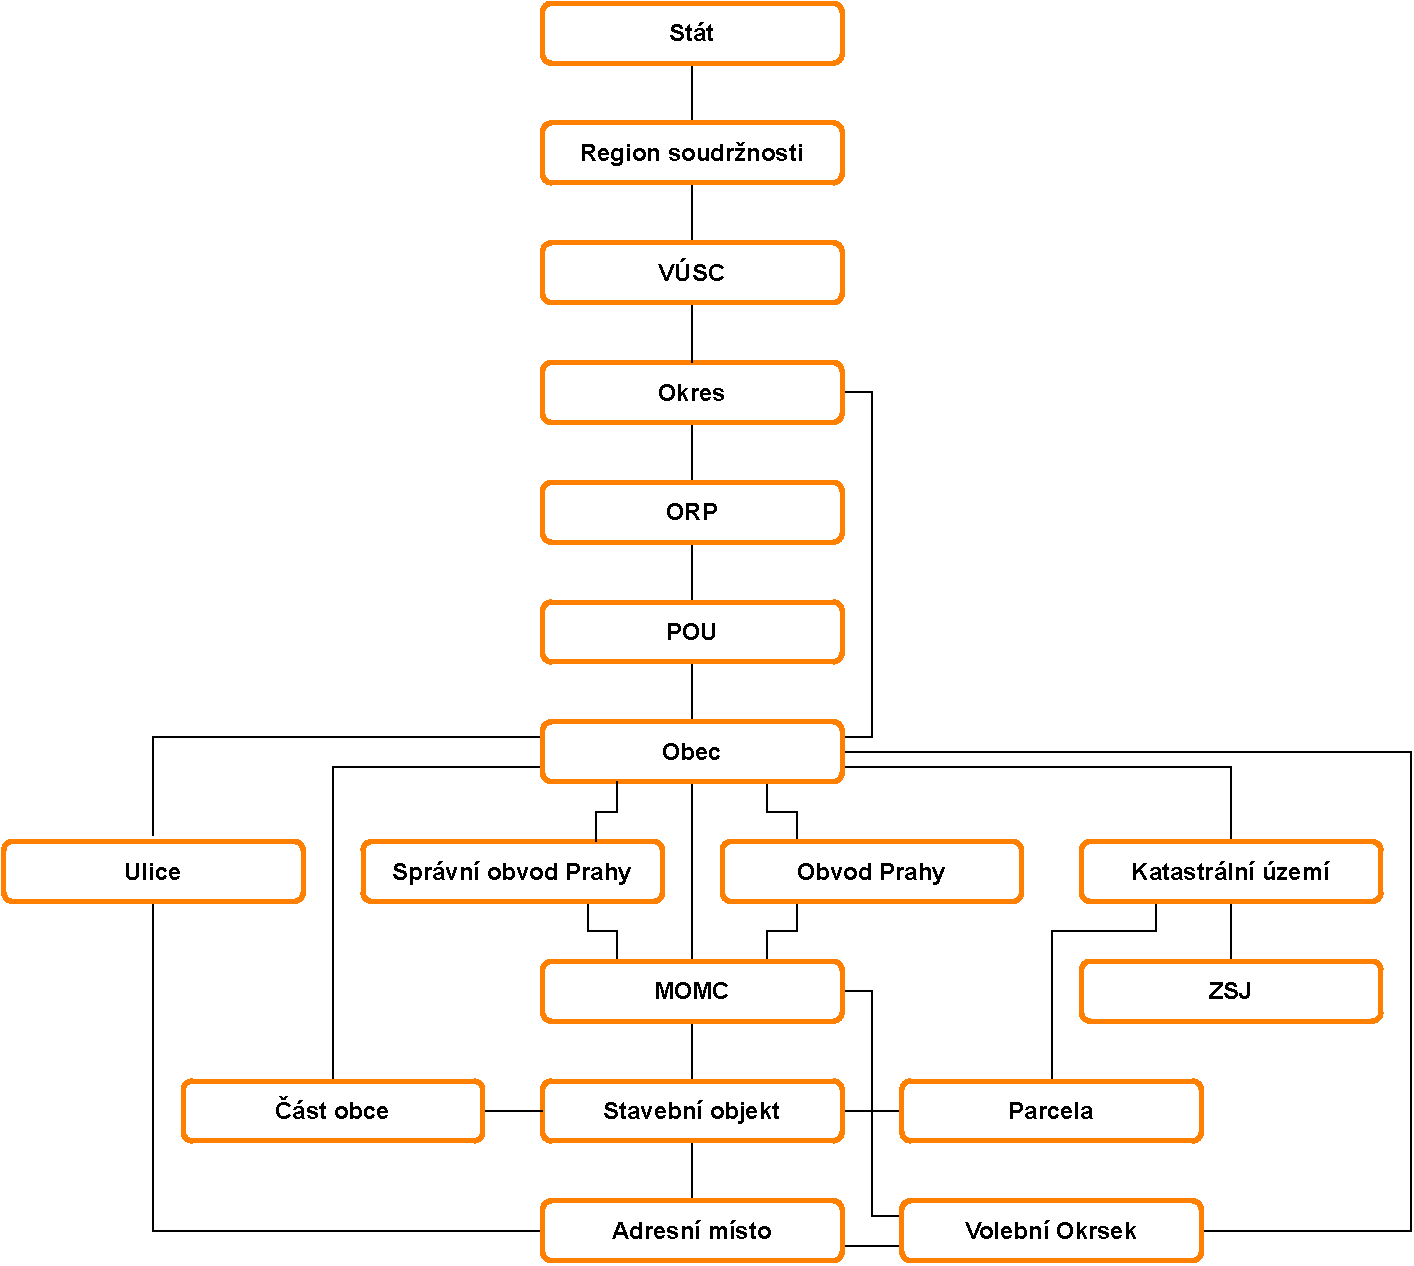
\includegraphics[width=\textwidth]{figures/ruian_diagram.pdf}
    \caption{Tabulky RÚIAN}
    \label{fig:ruian_tables}
\end{figure}